\documentclass[12pt,a4]{article}

\usepackage{graphicx,amsmath,amssymb,amsthm, boxedminipage}
\usepackage{algorithm}
\usepackage{algpseudocode}

\newtheorem{theorem}{Theorem}%[section]
\newtheorem{proposition}[theorem]{Proposition}
\newtheorem{lemma}[theorem]{Lemma}
\newtheorem{corollary}[theorem]{Corollary}
\newtheorem{definition}[theorem]{Definition}



\newcommand{\scalar}[2]{\ensuremath{\langle #1, #2\rangle}}
\newcommand{\floor}[1]{\left\lfloor #1 \right\rfloor}
\newcommand{\ceil}[1]{\left\lceil #1 \right\rceil}
\newcommand{\norm}[1]{\|#1\|}
\newcommand{\pfrac}[2]{\left(\frac{#1}{#2}\right)}
\newcommand{\nth}[1]{#1\textsuperscript{th}}

% \newcommand{\nth}[1]{#1\textsuperscript{th}}
\newcommand{\E}{\mathop{\mathbb{E\/}}}
\newcommand{\N}{\mathbb{N}}

\newcommand{\R}{\mathbb{R}}

\newtheorem{exercise}[theorem]{Exercise}
\newtheorem{exerciseD}[theorem]{*Exercise}
\newtheorem{exerciseDD}[theorem]{**Exercise}

\let\oldexercise\exercise
\renewcommand{\exercise}{\oldexercise\normalfont}

\let\oldexerciseD\exerciseD
\renewcommand{\exerciseD}{\oldexerciseD\normalfont}

\let\oldexerciseDD\exerciseDD
\renewcommand{\exerciseDD}{\oldexerciseDD\normalfont}


 
\begin{document}

\date{\today}
\author{NoCode}

\title{CS 217 -- Algorithm Design and Analysis \\ 
  \vspace{3mm}
    {\large	Shanghai Jiaotong University, Fall 2019\\}
}

\maketitle

\noindent
\setcounter{section}{2}

\section{Minimum Spanning Trees}

Throughout this assignment, let $G$ be a weighted graph, i.e., $G=(V,E,w)$ 
with $w: E \rightarrow \R^+$.
For $c \in \R$ and a weighted graph $G = (V,E,w)$, let
  $G_c := (V, \{e \in E \ | \ w(e) \leq c\})$. That is, $G_c$ is the
  subgraph of $G$ consisting of all edges of weight at most $c$.


\begin{exercise}
  Let $T$ be a minimum spanning tree of $G$, and let $c \in \R$.  Show that
  $T_c$ and $G_c$ have exactly the same connected components.  (That
  is, two vertices $u,v \in V$ are connected in $T_c$ if and only if
  they are connected in $G_c$).
  You are encouraged to draw pictures to illustrate your proof!
  
\begin{proof}
    It is obvious that if vertices $u,v\in V$ are connected in $T_c$, they will also be connected in $G_c$. So we need to prove that if vertices $u,v\in V$ are connected in $G_c$, they will also be connected in $T_c$.

    Suppose there is an edge $e$ in $G_c$ that connects $u$ and $v$, but $u$ and $v$ are not connected in $T_c$. Therefore, $e$ should be added to $T_c$ in order to construct a minimum spanning tree (otherwise, the tree we constructed can have a smaller edge cost), which forms a contradiction. So, $e$ must be in $T_c$ and $u,v$ must be connected.

    Thus, $T_c$ and $G_c$ have exactly the same connected components.
\end{proof}
  
\end{exercise}

\begin{exercise}
  For a weighted graph $G$, let $m_c(G) := | \{ e \in E(G) \ | \ w(e) \leq c\}|$, i.e.,
  the number of edges of weight at most $c$ (so $G_c$ has $m_c(G)$ edges).
  Let $T, T'$ be two minimum spanning trees of $G$. Show that
  $m_c(T) = m_c(T')$.
\end{exercise}
\paragraph{solution}

LEMMA: Any two minimum spanning tree have the same ordered edge weight list. (we sort the edge weight in $T, T'$ from small to large, and the two weight list are the same)

\paragraph{proof of the lemma} Suppose after sorting the edges in $T$ becomes $a_1, a_2, \cdots , a_m$, $w(a_1) \leq w(a_2) \leq \cdots \leq w(a_m)$, the 
edges in $T'$ becomes $b_1, b_2, \cdots , b_m$, $w(b_1) \leq w(b_2) \leq \cdots \leq w(b_m)$. Suppose $i$ is the first number that $a_i$ is the different edge with $b_i$.
We can suppose $w(a_i) \geq w(b_i)$.\\
case 1: $b_i$ is in $T$, so there must exist $j > i$ that $b_i = a_j$. In fact, we now have $w(b_i) = w(a_j) \geq w(a_i) \geq w(b_i)$, so $w(b_i) = w(a_j) = w(a_i)$. So we can change the position 
of $a_i$ and $a_j$ in $a_1, a_2, \cdots , a_m$, now $T$ and $T'$ have the same edge in the position i.\\
case 2: $b_i$ is not in $T$, so we can add $b_i$ to $T$ which will lead to a cycle. For $T$ is the minimum spanning tree, each edge in the cycle has a weight not less than $w(b_i)$, and there exists 
$a_j$ which is not in $T'$. So we have $w(a_j) \leq w(b_i)$ and $j>i$, so $w(bi)\leq w(ai)\leq w(aj)\leq w(bi)$, so $w(a_i) = w(a_j) = w(b_i)$. So we can replace $a_j$ with $b_i$ to let $T$ still a minimum
spanning tree, than this case turn to case 1.\\
According to the lemma, we can easily get $m_c(T) = m_c(T')$\\\\
below is another proof based on \testbf{Exercise 1}
\begin{proof}
    According to \textbf{Exercise 1.}, $T_c$, $T'_c$ and $G_c$ have exactly the same connected components. 
    So the number of connected components in $T_c$, $T'_c$ and $G_c$ should be the same.

    Since both $T$ and $T'$ are minimum spanning trees, all the connected components of $T_c$ and $T'_c$ should be trees. 

    Let $G$ has $n$ vertices, we can derive 
    
    $m_c(T) = m_c(T') = n - \mbox{ the number of connected components in } G_c$.
\end{proof}

\begin{exercise}
  Suppose $G$ is connected, and no two edges of $G$ have the same weight. 
  Show that $G$ has exactly one minimum spanning tree!
\end{exercise}

\paragraph{solution}
Suppose $T, T'$ are two minimum spanning trees of $G$, suppose $T$ has edges $E(T) = \{ e_1, e_2, \dots, e_m\}$ and $T'$ has edges $E(T') = \{e_1', e_2' \dots, e_m'\}$, the edges in set are arranged 
in weight from small to large. Suppose $k$ is the first number that
makes $e_k \neq e_k'$ which means $e_i = e_i'$ for all $i < k$. Now we can suppose that $w(e_k) < w(e_k')$, then we add $e_k$ to the $T'$, and now there exists a cycle in $T'$. And we can claim
that there must be at least one edge that larger than $e_k$, other than the cycle is composed with the edges among $e_1, e_2, \cdots, e_{k}$ which can lead to an cycle in $T$. So now we can delete 
an larger edge in this cycle to get another spanning tree
with smaller weight. So we get the contradiction, and the suppose are not true. So we showed that G has exactly one minimum spanning tree!


A {\em multigraph} is a graph that can have multiple edges, called
``parallel edges''. Without defining 
it formally, we illustrate it:
\begin{center}
  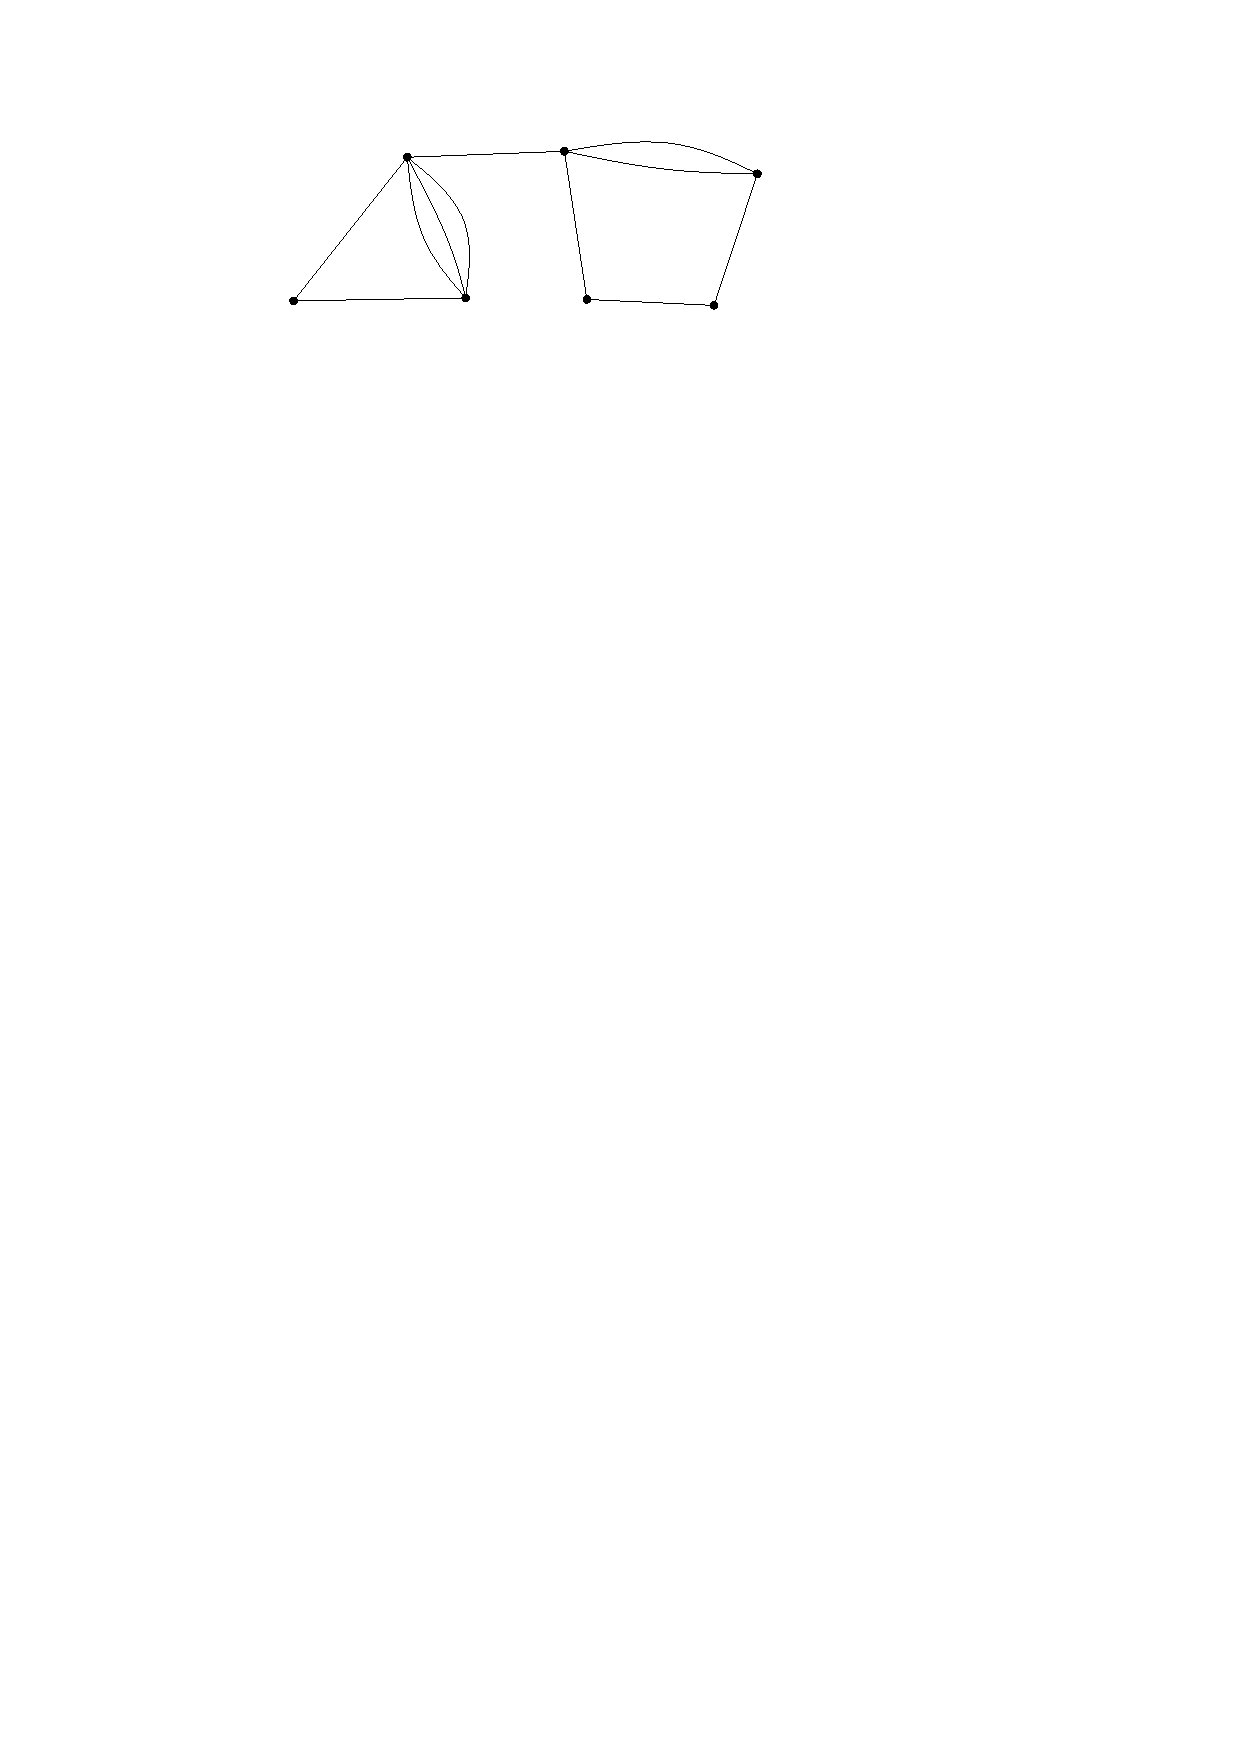
\includegraphics[width=0.6\textwidth]{figures/multigraph.pdf}\\
  A multigraph.
\end{center}
All other definitions, like connected components and spanning trees
are the same as for normal (simple) graphs. However,
when two spanning trees use different parallel edges, we consider them
different:
\begin{center}
  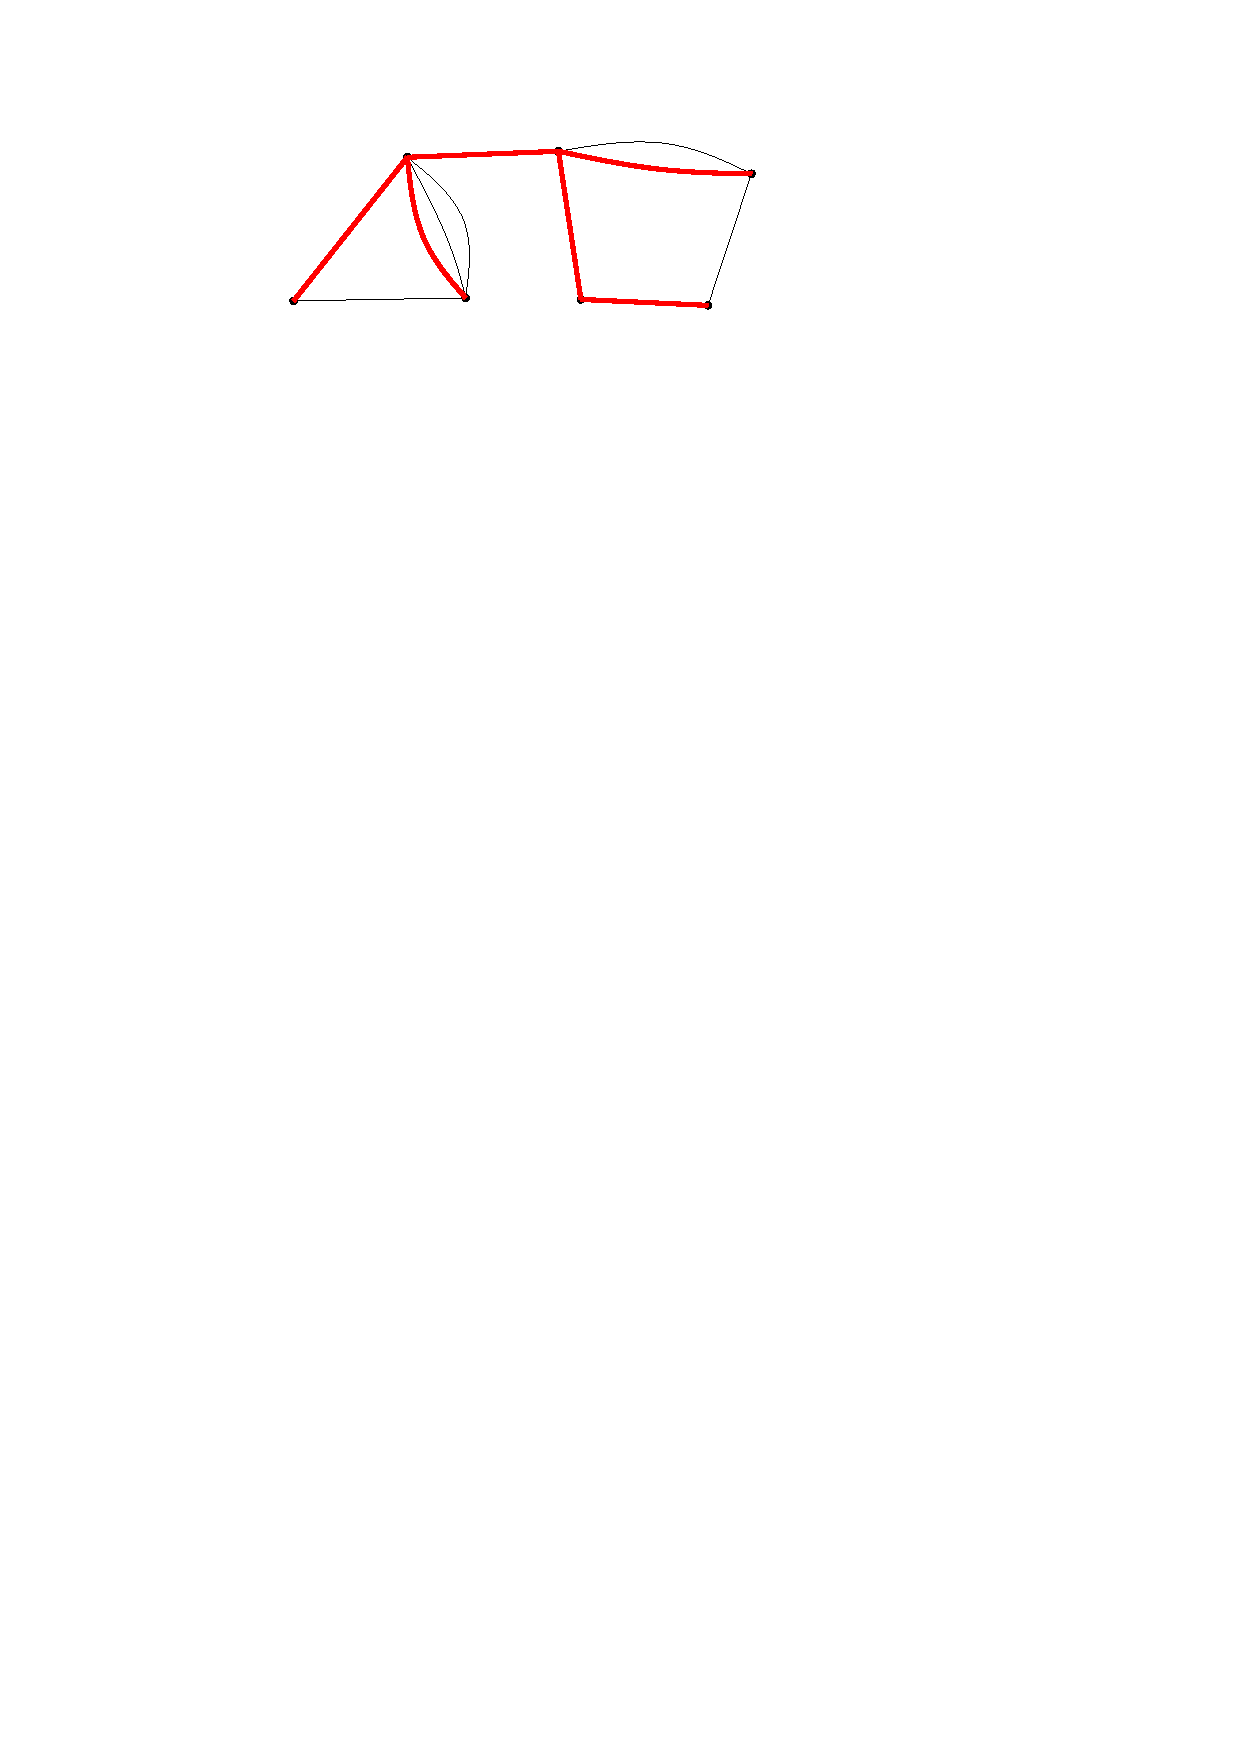
\includegraphics[width=0.4\textwidth]{figures/multigraph-forest.pdf} \hspace{2cm}
  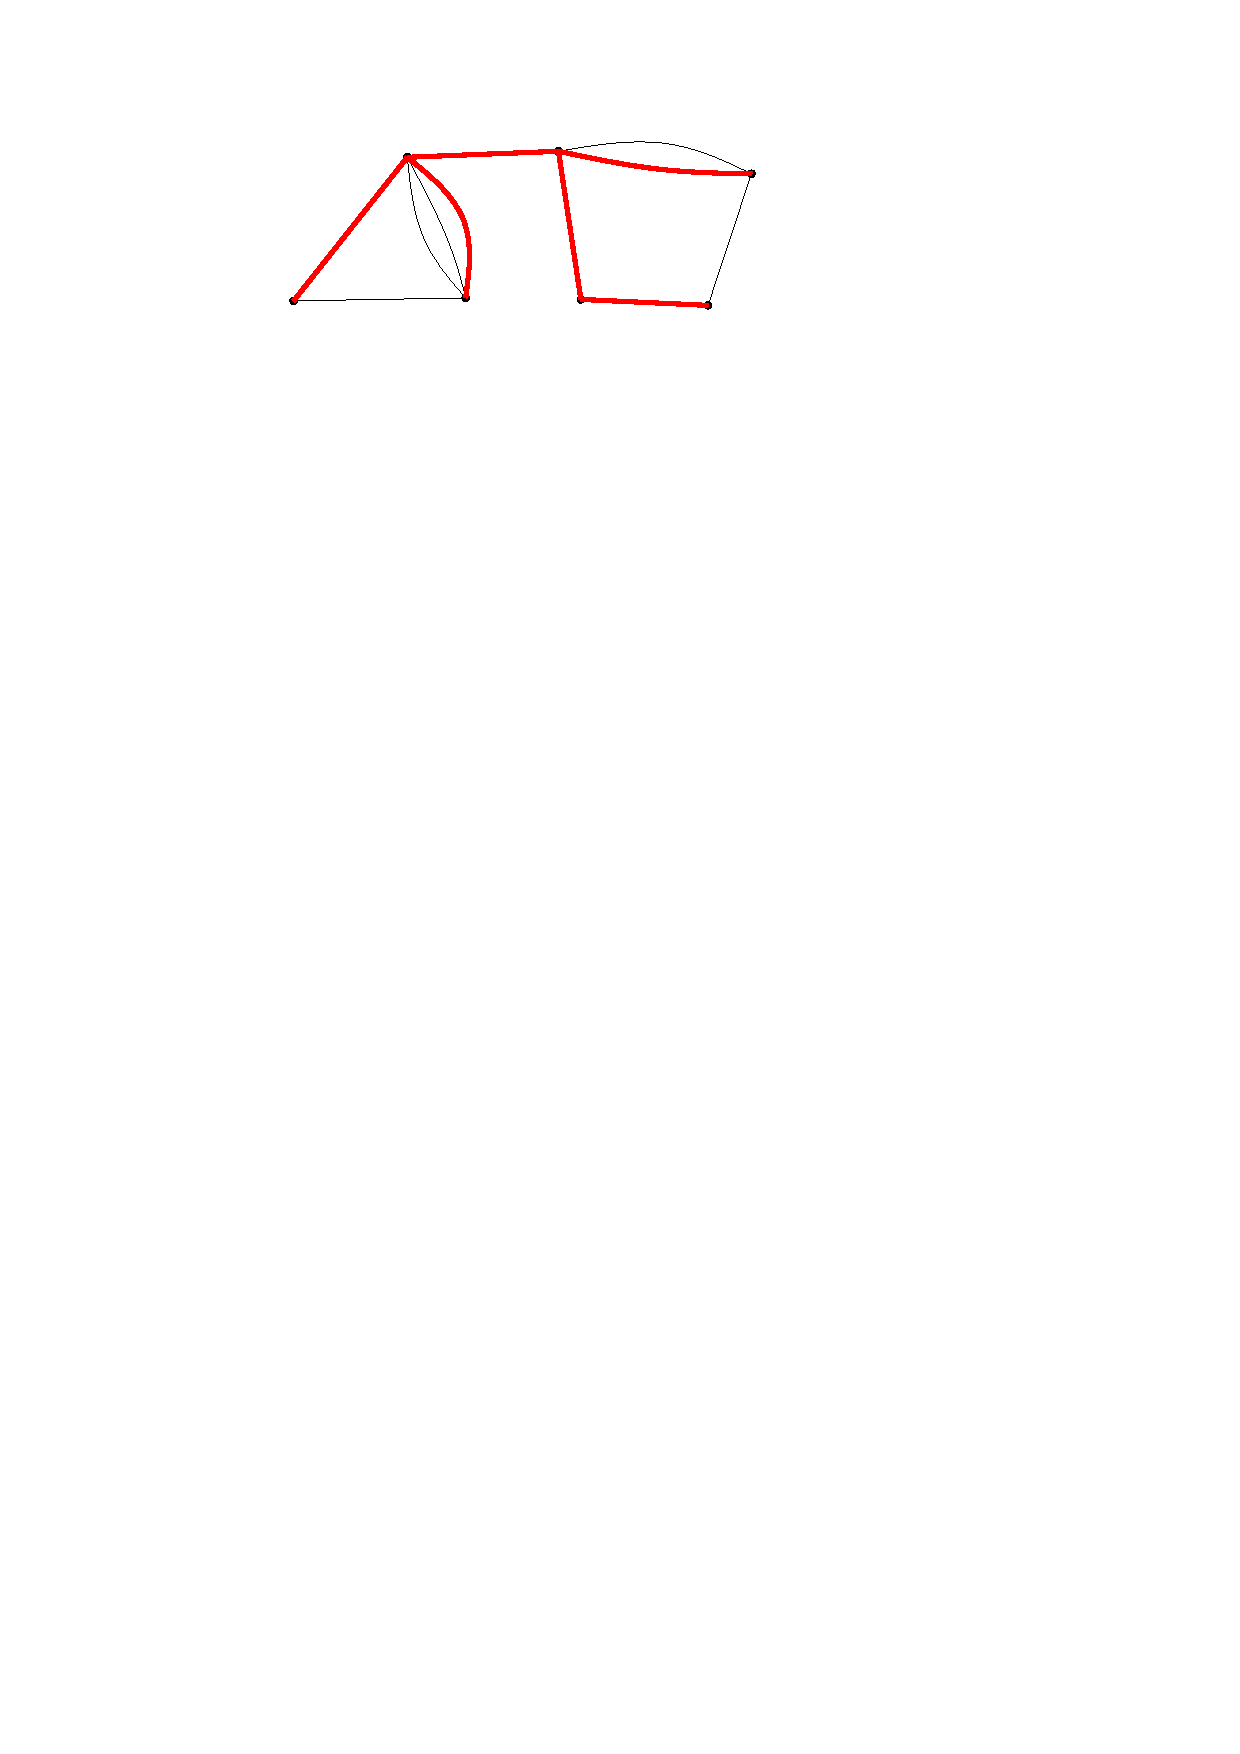
\includegraphics[width=0.4\textwidth]{figures/multigraph-forest-other.pdf} \\
  The same multigraph with two different spanning trees.
\end{center}


\begin{exercise}
  How many spanning trees does the above multigraph on 7 vertices have?
  Justify your answer!\\
  \paragraph{Solution}
  49.
  \paragraph{Proof} For an n-point cycle, taking $a_i$ as the number of edges between point $i$ and point $i+1$ ( or point n and point 1),the MST number of the graph is:
  \begin{align*}
    \sum_{i=1}^{n}\prod_{j=1,j!=i}^{n}a_j
  \end{align*}
  It's easy to show it considering the ways to get an MST without edges between point $i$ and point $i+1$.\\
  Then we can seperate the graph into two cycles, the three-point one has 7 ways to get an MST, and the four-point one has also 7 ways to get an MST. Apparently the edge linking the two graph has to be selected, so the total number of MST for the graph equal to the product of that of the subgraph, which means, $7\times7 = 49$.
\end{exercise}

\begin{exercise}
  Suppose you have a polynomial-time algorithm that, given a multigraph $H$,
  computes the number of spanning trees of $H$.
  Using this algorithm as a subroutine, design a polynomial-time algorithm
  that, given a weighted graph $G$, computes the number of 
  minimum spanning trees of $G$.

  \paragraph{Solution}
    Consider $A$ is MST of $G$, it has $k$ edges weighted $v$. If we replace 
   this $k$ edges by other $k$ edges weighted $v$ and does not generate cycle 
   , we call the new graph is $B$, then $B$ is also a legal MST. Because
   according to \textbf{Exercise 1}, any two MST of $G$ 
   have the same number of edges with weight of v, and 
   according to \textbf{Exercise 2}. $G_c$ and $A_c$ have the same
   connected components. So we can design the algorithm from the idea:

   \begin{algorithm}
    \caption{Computes the number of MST of $G$}
    \begin{algorithmic}[1]
    \Procedure{MinimumSpanningTreeCount}{$G$}
        \State T := $\textsc{Kruskal}(G)$
        \State E := Edge set of T
        \State ans := 1
        \For{e $\in$ E}
            \State $\omega$ := weight of e
            \If {$\omega$ has not been proccessed}
                \State $W$ := Set of edges in T with weight $\omega$        
                \State $G'$ := $(V, E / W)$
                \State $C$ := Number of connected component if $G'$
                \State $H$ := Empty graph with $C$ vertices.
                \For{$w \in W$}
                    \If {$w$ connect two connected component $u,v \in G'$}
                        \State Add edge $\{ u, v \}$ to $H$
                    \EndIf 
                \EndFor
                \State ans := ans $\cdot \textsc{SpanningTreeCount}(H)$
            \EndIf
        \EndFor
        \State \Return ans
    \EndProcedure
    \end{algorithmic}
\end{algorithm}
\end{exercise}

In the algorithm, we generate a MST by \textsc{Kruskal}, then We can know how many times the edge of a certain weight appears. For certain weight $\omega$, the algorithm remove all edges with weight $\omega$, then treat a connected block as a vertex. Then find all 
spanning tree of the new graph. and use the principle of multiplication to get the answer.


\end{document}
